\subsection{Top-Level Overview Diagram of the alamSYS and Its Interactions to External Systems}
\label{subsec:top_level_overview}

Figure \ref{fig:system_overview} shows the top-level overview of the 
alamSYS and its interactions to any third-party or external applications.

% Sytem Overview Diagram
\begin{figure}[ht]
    \centering
    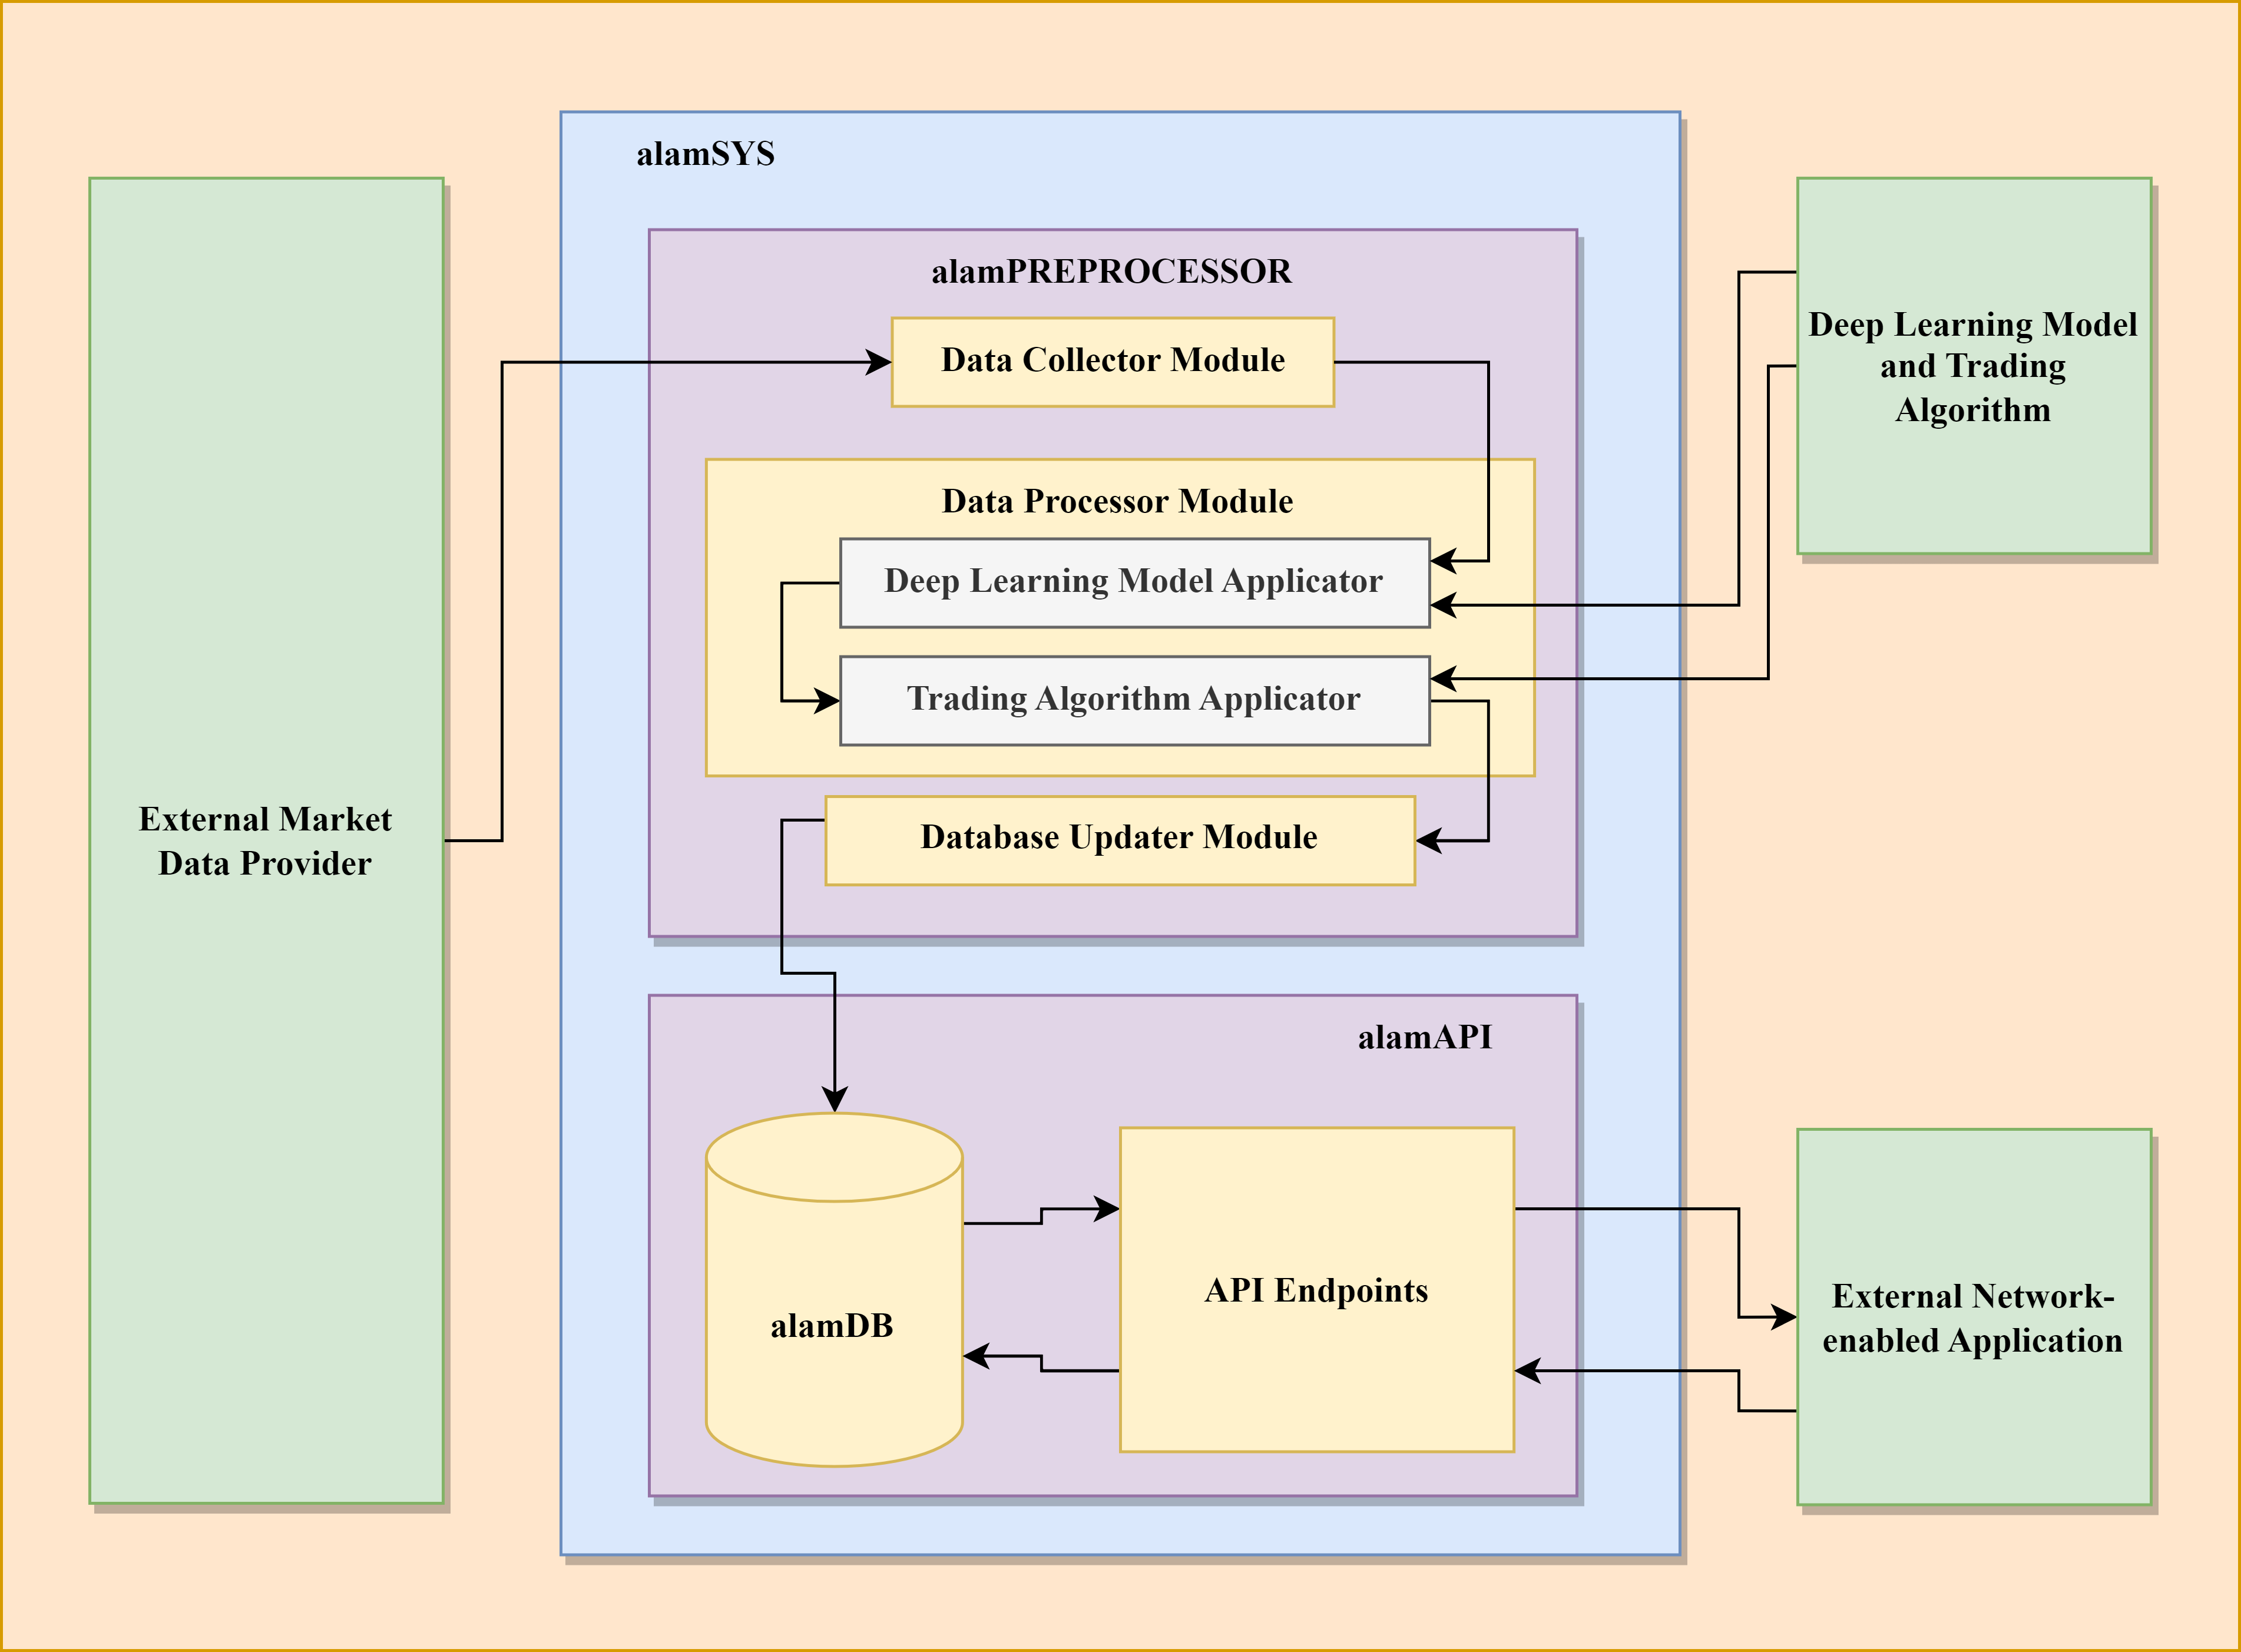
\includegraphics[width=1\textwidth]{./assets/Chapter_3/SystemOverview.png}
    \caption{Top-Level Overview of the alamSYS and Interactions with External Applications/Systems}
    \label{fig:system_overview}
\end{figure}
\FloatBarrier

As shown from the figure above, the alamSYS is connected to three external 
entities: (1) External Market Data Provider, which provides the system with the 
needed historical market data; (2) Machine Learning Model or Trading Algorithm, 
in the case of this special problem, a machine learning model will be developed and 
will be utilized by the system, however as previously discussed the system is 
created to accept any other machine learning model or proprietary trading algorithms 
that other developers may or want to develop in the future; and 
(3) External Application, which can be a web-based or mobile-based application, that
will utilize and showcase the functionalities provided by the alamSYS, through the
API endpoints.
\hfill \\

On the middle of the diagram the alamSYS is observed to have three main components, 
namely, (1) Pre-processor, which is further divided into sub-components: 
(a) Data Collector, which collects the data from the external market data provider; 
(b) Pre-Database Processor, which processes the historical market data collected by 
applying the developed machine learning model and sending it to the database updater 
module; (2) Database, which is based on MongoDB, which is a document-based and non-relational 
database; finally, the database is connected to the (3) API endpoints which processes 
the request and responses of the system to any external application connected to the 
API via a network.